\documentclass[border=0.2cm]{standalone}

\renewcommand{\familydefault}{cmtt}
\usepackage{graphicx}
\usepackage{sectsty}
\usepackage{lipsum}
\usepackage{cases}
\usepackage{tikz}
\usetikzlibrary{shapes.geometric}
\usetikzlibrary{calc}
\usetikzlibrary{arrows}
\usetikzlibrary{decorations.pathreplacing}
\usetikzlibrary{arrows.meta}


\begin{document}
    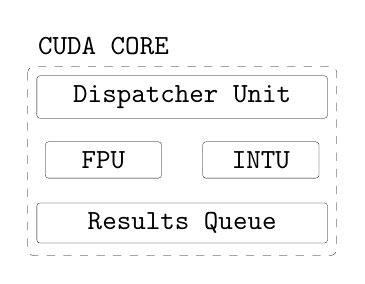
\begin{tikzpicture}[state/.style={rectangle, draw, rotate=90, minimum width=80pt}]

		\node (ccore) at (0,0) {CUDA CORE};

		\node[rectangle,draw, line width=0.1pt, rounded corners=0.25ex, minimum width=10em] (dispatch) at (1,-0.65) {Dispatcher Unit};
		\node[rectangle,draw, line width=0.1pt, rounded corners=0.25ex, minimum width=4em] (fpu) at (0,-1.45) {FPU};
		\node[rectangle,draw, line width=0.1pt, rounded corners=0.25ex, minimum width=4em] (intu) at (2,-1.45) {INTU};
		\node[rectangle,draw, line width=0.1pt, rounded corners=0.25ex, minimum width=10em] (res) at (1,-2.25) {Results Queue};

		\draw [dashed, line width=0.1pt, rounded corners=0.5ex] ($(ccore.north west)+(0, -0.5)$) rectangle ($(ccore.north east)+(2,-2.9)$);
    \end{tikzpicture}
\end{document}
